\documentclass{beamer}

% This file is a solution template for:

% - Giving a talk on some subject.
% - The talk is between 15min and 45min long.
% - Style is ornate.



% Copyright 2004 by Till Tantau <tantau@users.sourceforge.net>.
%
% In principle, this file can be redistributed and/or modified under
% the terms of the GNU Public License, version 2.
%
% However, this file is supposed to be a template to be modified
% for your own needs. For this reason, if you use this file as a
% template and not specifically distribute it as part of a another
% package/program, I grant the extra permission to freely copy and
% modify this file as you see fit and even to delete this copyright
% notice. 


\mode<presentation>
{
  \usetheme[height=12mm]{Rochester}
  % or ...%

  \setbeamercovered{transparent}
%  % or whatever (possibly just delete it)
}


\usepackage[brazil]{babel}
% or whatever

% or whatever
%\usepackage{graphics}
\usepackage{times}
\usepackage[utf8]{inputenc}
\usepackage{url}

\newcommand{\nektar}{\ensuremath{\mathcal{N}\varepsilon \kappa \tau \alpha r}}
\newcommand{\ordem}[1]{ \ensuremath{\mathcal{O}[#1]}}
\newcommand{\pr}[1]{\ensuremath{ \mathbf{#1}}}    % \pr vem de preto
\newcommand{\etal}{\emph{et al.}}
\newcommand{\jac}[4]{ \ensuremath{ P_{#2}^{#3,#4}(#1) }}
\newcommand{\der}[2]{\ensuremath{ \frac{\partial #1}{\partial #2}}}
\newcommand{\convect}[2]{\ensuremath{ #1 \cdot \nabla #2}}
\newcommand{\R}{\ensuremath{ Re }}
\newcommand{\St}{\ensuremath{ St }}
\newcommand{\cpb}{\ensuremath{ C_{pb}}}
\newcommand{\transf}[3]{\ensuremath{ \int_{-\infty}^\infty #3\: e^{i #2 #1}\: d #2}}
\newcommand\clrms{\ensuremath{\sqrt{\overline{C_L^2}}}}
\newcommand{\epseudo}{\ensuremath{ \epsilon-\text{pseudospectro}}}
\newcommand{\lra}{\ensuremath{\longrightarrow}}

\newcommand{\wt}[1]{\ensuremath{\widetilde{#1}}}
\newcommand{\mcal}[1]{\ensuremath{\mathcal{#1}}}

\newcommand{\ol}[1]{\ensuremath{\overline{#1}}}
\newcommand{\us}{\ensuremath{u_*}}

\newcommand{\p}[1]{\ensuremath{ \mathbf{#1}}}    % \pr vem de preto
\newcommand{\qrq}{\ensuremath{\quad\lra\quad}}
\newcommand{\qqrq}{\ensuremath{\qquad\lra\qquad}}
\newcommand{\pd}{\ensuremath{\partial}}
\newcommand{\bigO}[1]{\ensuremath{\mathcal{O}\left(#1\right)}}


\title{Modelos, Escalas e Semelhança}


\author{Paulo Jabardo}

\titlegraphic{
\includegraphics[width=4cm]{figuras/logo-ipt.png}}%}
%   \includegraphics[width=2cm]{fig
%}
\date{24-11-2023}





\begin{document}
\maketitle
\begin{frame}{Análise Dimensional}
  
  \begin{itemize}
  \item As leis físicas não podem depender do sistema de unidades
  \item Todos os sistemas de unidades são equivalentes
  \item As dimensões de uma grandeza são monômios
  \item Teorema do $\Pi$s de Buckingham
  \item Escolher a classe do sistema de unidades
  \item Lucro???
  \end{itemize}
\end{frame}

\begin{frame}{GI Taylor: explosão nuclear}
  
  \begin{itemize}
  \item 1940: Será que uma explosão com uma grande quantidade de energia seria efetiva?
  \item Um renomado especialista disse que o efeito mecânico não seria muito maior: perda por radiação.
  \item G. I. Taylor entra na jogada
  \item Resumindo: pode fazer que vai funcionar!
  \item 1950: Taylor publica artigo com dados de energia das bombas atômicas
  \item Visita da CIA/MI6/etc
\end{itemize}
  
\end{frame}

\begin{frame}{O que fez G. I. Taylor?}
  O que acontece com o ar ambiente após a explosão?
  \begin{itemize}
  \item Após um curto tempo uma forte onda de choque aparece
  \item Movimento com simetria esférica
  \item O que envolve?
    \begin{itemize}
    \item Equação da conservação de massa
    \item Equação da conservação da quantidade de movimento
    \item Equação da conservação de energia
    \end{itemize}
  \item Problema complexo...
  \end{itemize}

 
\end{frame}

\begin{frame}{Problema ideal}
  \begin{itemize}
  \item Quantidade finita de energia é liberada de maneira concentrada: $r_0 \equiv 0$
  \item Pressão na onde de choque muito maior que a pressão ambiente $p_0$
  \end{itemize}
  A questão é o raio da frente da onda $r_f$ depende de quê?
  \begin{enumerate}
  \item $E$ energia total da explosão
  \item $\rho_0$ densidade do ar ambiente
  \item $t$ tempo a partir do instante da explosão
  \item $r_0$ raio inicial da onda de choque
  \item $p_0$ Pressão ambiente
  \item $\gamma$ Coeficiente adiabático
  \end{enumerate}

\end{frame}

\begin{frame}{Classe e unidades}
  \begin{itemize}
  \item \[ [E] = J = \frac{kg\cdot m^2}{s^2}\]
  \item \[ [\rho_0] = \frac{kg}{m^3} \]
  \item \[ [t] = s \]
  \item \[ [p_0] = \frac{kg}{m\cdot s^2} \]
  \end{itemize}

  \[
  r_f = r_f\left(t, r_0, p_0, \rho_0, E, \gamma\right)
  \]
  Chegamos a algo bem complicado...
\end{frame}

\begin{frame}{E se desprezarmos $r_0$ e $p_0$?}
  \[
  r_f = r_f \left(t, \rho_0, E, \gamma\right)
  \]
  
  Escala de comprimento:
  \[
  R = \left( \frac{E \cdot t^2}{\rho_0} \right)^\frac{1}{5}
  \]

  Temos
  \[
  I = \frac{r_f}{R} = F\left(R, t, \rho_0, \gamma\right)
  \]
  Três argumentos de $F$ têm dimensões  independentes. Variando a unidade de $t$, nada muda! Mesma coisa se mudarmos a unidade de massa! Variando a unidade de comprimento, $r_f$ varia mas não $I$

  \[
  r_f = C(\gamma)\left( \frac{E \cdot t^2}{\rho_0} \right)^\frac{1}{5}
  \]
  
\end{frame}

\begin{frame}{Vídeo da explosão}
  \centering
  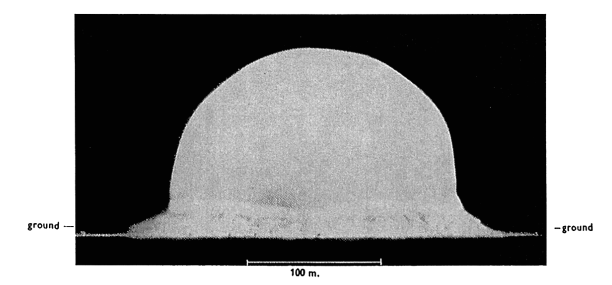
\includegraphics[width=\textwidth]{./figuras/explosao.png}
\end{frame}


\begin{frame}{Será que o modelo funciona?}
  \centering
  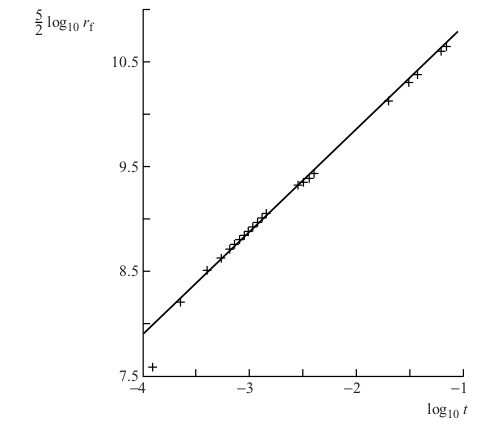
\includegraphics[height=0.95\textheight]{./figuras/explosao-raio.png}
\end{frame}

\begin{frame}{E as outras grandezas na onda de choque?}
  \begin{itemize}
  \item \[ p_f = C_p(\gamma) \left( \frac{E \cdot t^2}{\rho_0} \right)^\frac{1}{5} \]
  \item \[ \rho_f = C_\rho(\gamma) \rho_0 \]
  \item \[ u_f = C_u(\gamma)\left( \frac{E}{t^3\rho_0} \right)^\frac{1}{5} \]
  \end{itemize}

\end{frame}

\begin{frame}{Mas e dentro da onda de choque?}
  Autosemelhança!
  \begin{itemize}
  \item \[ p = p_f P\left(\frac{r}{r_f}, \gamma\right) \]
  \item \[ \rho = \rho_f R\left(\frac{r}{r_f}, \gamma\right) \]
  \item \[ u = u_f V\left(\frac{r}{r_f}, \gamma\right) \]
\end{itemize}
\end{frame}


\begin{frame}{Pêndulo simples}
  Qual o período $\theta$ de um pêndulo de comprimento $l$, massa $m$ e aceleração da gravidade $g$?

  \[
    [\theta] = T \qquad [l] = L \qquad [m] = M \qquad [g] = LT^{-2}
  \]

  $n=k=3$, portanto temos apenas 1 adimensional:
  \[
  \Pi = \frac{\theta}{l^{1/2}g^{-1/2}} \qrq \theta = const \cdot \sqrt{\frac{l}{g}}
  \]
  
  
\end{frame}

\begin{frame}{Vazão em um vertedouro}
  \centering
  \includegraphics[width=0.75\textwidth]{./figuras/vertedouro.png}
\end{frame}

\begin{frame}{Vertedouro: parâmetros e dimensões}
  \[
  Q = f(g,h,\alpha)
  \]
  \begin{itemize}
  \item $[Q] = L^3/T$, Vazão de fluido
  \item $[g] = L/T^2$, aceleração da gravidade
  \item $[h] = L$, nível da água
  \item $[\alpha] = 1$, ângulo do ``V''
  \end{itemize}

  E a viscosidade?
\end{frame}

\begin{frame}{Vertedouro}
  \[
  \begin{aligned}
    \Pi_1 &= \alpha\\
    \Pi_2 &= \frac{Q}{g^{1/2}\cdot h^{5/2}}\\
    \Pi_2 &= C(\Pi_1) = C(\alpha)\\
  \end{aligned}
  \]

  \[
  Q = C(\alpha)\cdot \sqrt{g} \cdot h^{5/2}
  \]
  Norma ISO-1438:2008, equação de Kindsvater-Shen:
  \[
  Q = C_d\frac{8}{15}\tan\frac{\alpha}{2}\sqrt{2g}h^{5/2} \qquad C_d = f\left(\frac{h}{p}, \frac{p}{B}, \alpha\right)
  \]
  
  
\end{frame}

\begin{frame}{Gradiente de pressão em tubulação}
  \[
  \frac{dp}{dx} = f(U, D, \rho, \mu)
  \]

  As dimensões:
  \[
  \left[\frac{dp}{dx}\right] = \frac{M}{L^2T^2}, \quad [U] = \frac{L}{T}, \quad [D] = L, \quad [\rho] = \frac{M}{L^3}, \quad [\mu] = \frac{M}{LT}
  \]

  $k=3$, $m=1$:
  \[
  \left[\frac{dp}{dx}\right] = [U]^2[D]^{-1}[\rho] \qrq \Pi = \frac{dp/dx}{U^2D^-{-1}\rho}
  \]
  \[
    [\mu] = [U][D][\rho] \qrq \Pi_1 = \frac{\mu}{\rho U D} = \frac{1}{Re}
    \]

    \[
    \frac{dp}{dx} = \frac{\Delta P}{\Delta x} = \frac{U^2}{D} \rho \Phi\left(\frac{\mu}{\rho U D}\right)
    \]
    
        
  
\end{frame}

\begin{frame}{Remo (McMahon, 1971)}
  Tempo de corrida de barcos a remo com número variável de remadores. Hipóteses:
  \begin{enumerate}
  \item Semelhança entre barcos
  \item Volume deslocado por cada remador $G$ é constante
  \item Potência por remador é constante e o mesmo para todas as classes
  \item O que impede o deslocamento é a força de arrasto viscosa. Ondas são desprezadas: potência de arrasto: $P = \lambda \rho v^3 l^2 = A\cdot N$
  \end{enumerate}
  A velocidade depende dos parâmetros $N$, $A$, $G$, e $\rho$
\end{frame}

\begin{frame}{Parâmetros e dimensões}
  \[
  v = v(N, A, G, \rho)
  \]
  Dimensões
  \[
    [v] = V, \quad [G] = \frac{L^3}{N}, \quad [A] = \frac{R V^3 L^2}{N}, \quad [\rho] = R, \quad [N] = N
    \]

    \[
    \Pi = \frac{G^{2/9}\rho^{1/3} v }{A^{1/3} N^{1/9}} \quad\longrightarrow\quad v = const \cdot \frac{A^{1/3}}{\rho^{1/3}G^{2/9}}\cdot N^{1/9}
    \]
    
  
\end{frame}

\begin{frame}{Resultados em várias competições}
  \centering
  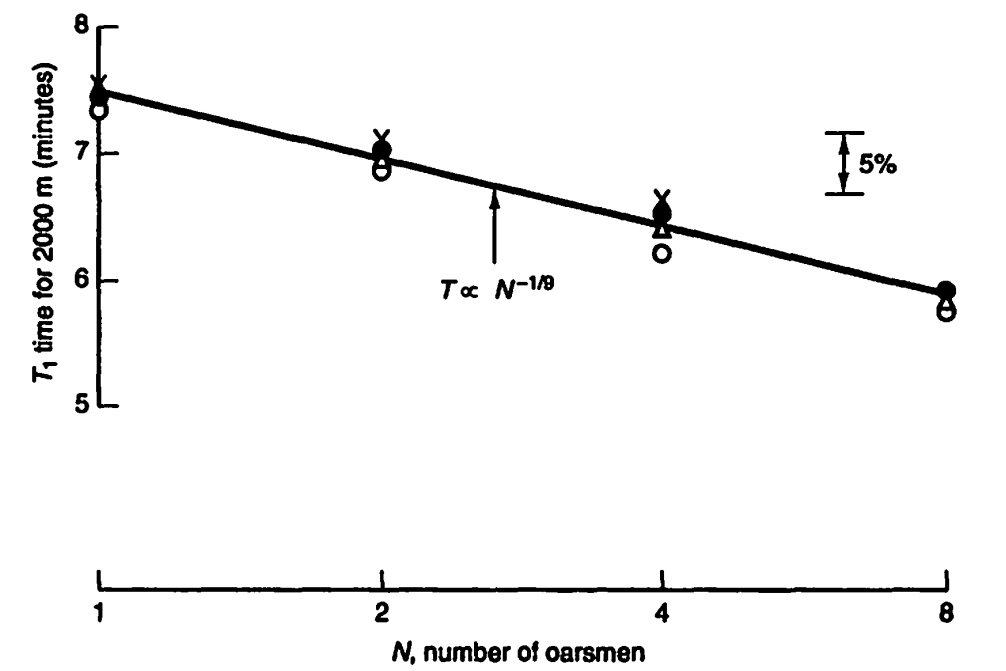
\includegraphics[width=0.95\textwidth]{./figuras/remo.png}
\end{frame}


\end{document}

\begin{frame}{}
\end{frame}

\begin{itemize}
\end{itemize}
